\documentclass{article}
\usepackage[activeacute,spanish]{babel}
\usepackage[latin1]{inputenc}
\usepackage{amssymb,amsmath}
\usepackage{amsthm}  
\usepackage{supertabular,float}
\usepackage[demo]{graphicx}
\usepackage[all]{xy}
\usepackage{tikz}
\usetikzlibrary{calc,trees,positioning,arrows,chains,shapes.geometric,
decorations.pathreplacing,decorations.pathmorphing,shapes,%
matrix,shapes.symbols,plotmarks,decorations.markings,shadows}
%%%%%% conjuntos numericos %%%%%%%%
\makeatletter
\gdef\Re{\relax\ifmmode I\hskip -3\p@ R\else
    \hbox{$I\hskip -3\p@ R$}\fi} %real
\gdef\na{\relax\ifmmode I\hskip -3\p@ N\else
    \hbox{$I\hskip -3\p@ N$}\fi} %natural
\gdef\en{\relax\ifmmode Z\hskip -4.8\p@ Z\else
    \hbox{$Z\hskip -4.8\p@ Z$}\fi} %enteros
\gdef\co{\relax\ifmmode C\hskip-4.8\p@\vrule \@height 5.8\p@ \@depth\z@
    \hskip 6.3\p@\else
    \hbox{$C\hskip-4.8\p@\vrule \@height 5.8\p@ \@depth\z@ \hskip 6.3\p@$}\fi}%complejo
\gdef\ra{\relax\ifmmode Q\hskip-5.0\p@\vrule
          \@height 6.0\p@ \@depth \z@ \hskip 6\p@\else
    \hbox{$Q\hskip-5.0\p@\vrule \@height 6.0\p@ \@depth \z@ \hskip 6\p@$}\fi}%racional
\gdef\ir{\relax\ifmmode I\hskip -3\p@ H\else
    \hbox{$I\hskip -3\p@ H$}\fi} %irracional
\gdef\ir{\relax\ifmmode I\hskip -3\p@ K\else
    \hbox{$I\hskip -3\p@ K$}\fi}
    \makeatother
    %%%%%%%%%%%%%%%%%%%%%%%
   \newcommand{\C}{\mathbb{C}}
\newcommand{\R}{\mathbb{R}}
\newcommand{\K}{\mathbb{K}}
\newcommand{\N}{\mathbb{N}}
\newcommand{\Z}{\mathbb{Z}}
\newcommand{\Q}{\mathbb{Q}}
\newcommand{\lin}{{\rm lin }}
\newcommand{\pr}{\partial}
\newcommand{\Li}{\mathcal{L}}
\newcommand{\Nu}{\mathcal{N}}
\newcommand{\B}{\mathfrak{B}}
\newcommand{\sgn}{{\rm sgn }}
\newcommand{\gra}{\nabla}
\newcommand{\dv}{\mathrm{ \, div \, }}
\newcommand{\dx}{\,\mathrm{d}x}
\newcommand{\re}{ \tfrac{1}{\mathrm{Re} } \,}
\begin{document}
\begin{figure}[ht]
  \fbox{\begin{minipage}[t]{150pt}
    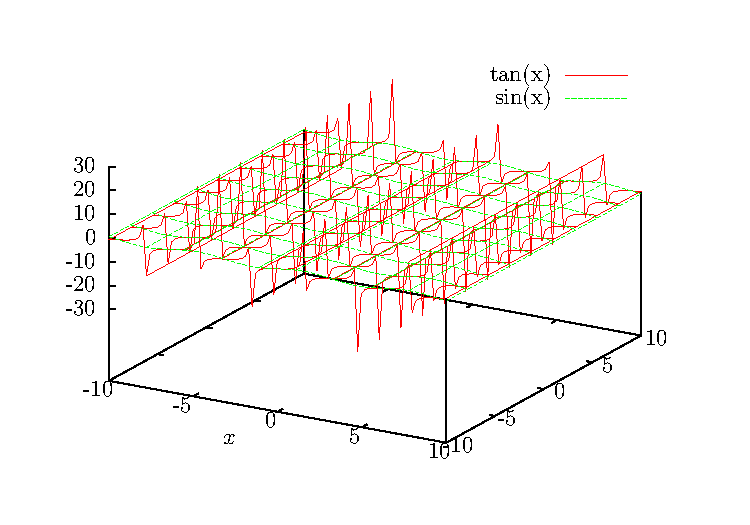
\includegraphics[height=100pt,width=150pt]{test}
  \end{minipage}}
  \hfill
  \fbox{\begin{minipage}[t]{150pt}
    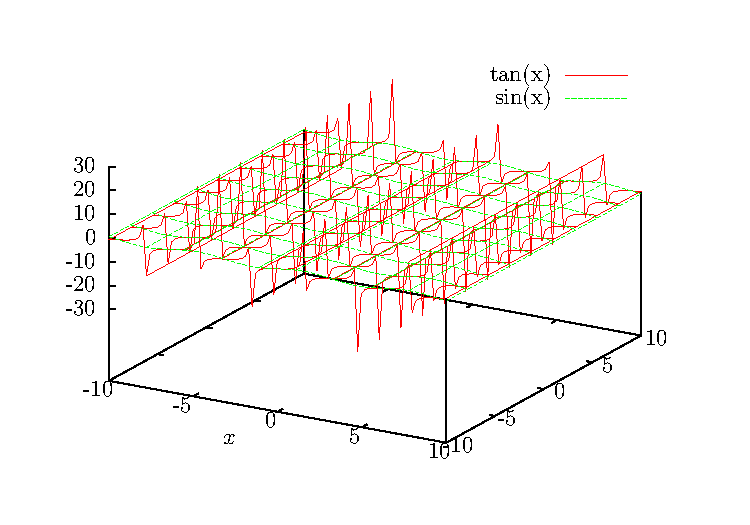
\includegraphics[height=60pt,width=150pt]{test}
  \end{minipage}}
\end{figure}
\begin{equation}
\xymatrix{
X \ar[r]^f & Y \ar[d]^\psi \\
X/R \ar[u]^\varphi & Y/Q \ar[l]_{\bar{f}}}
\end{equation}
%\tikzset{node distance=2cm, auto}
\begin{tikzpicture}[node distance=1.5cm, auto]
  \node (C) {$C$};
  \node (P) [below of=C] {$\prod_{i \in I} A_i$};
  \node (Ai) [right of=P] {$A_i$};
  \draw[->] (C) to node {$f_i$} (Ai);
  \draw[->, dashed] (C) to node [swap] {$\langle f_i \rangle_{i \in I}$} (P);
  \draw[->] (P) to node [swap] {$\pi_i$} (Ai);
\end{tikzpicture}
\begin{tikzpicture}[description/.style={fill=white,inner sep=2pt}]
\matrix (m) [matrix of math nodes, row sep=3em,
column sep=2.5em, text height=1.5ex, text depth=0.25ex]
{ A &|[red]|  B \\
 C & D\\ };
\path[->,font=\scriptsize]
(m-1-1) edge node[auto] {$ \varphi $} (m-1-2)
edge node[description] {$ \Psi $} (m-2-1)
(m-2-1) edge node[auto] {$ \Phi $} (m-2-2)
(m-1-2)edge node[auto] {$ \Phi $} (m-2-2);
\end{tikzpicture}\\
\begin{center}
\begin{tikzpicture}[description/.style={fill=white,inner sep=2pt}]
\matrix (m) [matrix of math nodes, row sep=3em,
column sep=2.5em, text height=1.5ex, text depth=0.25ex]
{|[red]| \Re &|[red]|  \Re\\
 |[red]|\Re &|[red]| \Re\\ };
\path[->,font=\scriptsize,blue,thick]
(m-1-1) edge[thick] node[auto] {$f$} (m-1-2)
edge[thick] node[ left] {$ \Psi $} (m-2-1)
(m-2-1) edge[thick] node[auto] {$g$} (m-2-2)
(m-1-2)edge[thick] node[auto] {$ \Phi $} (m-2-2);
\end{tikzpicture}
\end{center}
\begin{tikzpicture}[node distance=1.5cm, auto,thick,blue]
  \node (C)[red] {\Re};
  \node (P) [below of=C,red] {\Re};
  \node (Ai) [right of=P,red] {\Re};
  \node(D)[right of=C,red]{\Re};
  \draw[->] (C) to node {$f$} (D);
  \draw[->] (C) to node [swap] {$ \Psi $} (P);
  \draw[->] (P) to node  {$g$} (Ai);
  \draw[->] (D) to node  {$ \Phi $} (Ai);
\end{tikzpicture}
\begin{tikzpicture}[description/.style={fill=white,inner sep=2pt}]
\matrix (m) [matrix of math nodes, row sep=3em,
column sep=2.5em, text height=1.5ex, text depth=0.25ex]
{|[red]| \R &|[red]|  \R\\
 |[red]|\R &|[red]| \R\\ };
\path[->,blue,thick]
(m-1-1) edge[thick] node[auto] {$f$} (m-1-2)
edge[thick] node[ left] {$ \Psi $} (m-2-1)
(m-2-1) edge[thick] node[auto] {$g$} (m-2-2)
(m-1-2)edge[thick] node[auto] {$ \Phi $} (m-2-2);
\end{tikzpicture}
$ \R\, \K\, \N\, \Q\, \lim\, \pr\, \Li\, \Nu\, \B\, \sgn\, \dv\,$\\
$\dx\, \re\, \Z\, \C\,$ \ir\, \ra\, \co\, \en\, \na\,\Re\,

\end{document}
